\documentclass[answers]{exam}
\usepackage{../MT2023}
\usepackage{graphicx}
\graphicspath{ {./images} }

\title{Probability -- Sheet 5}
\author{YOUR NAME HERE :)}
\date{Michaelmas Term 2023}


\begin{document}
\maketitle
\begin{questions}

\question%1
A bug jumps around the vertices of a triangle. At every jump, it moves from its current position to either of the other two vertices with probability $1 / 2$ each (independently of how it arrived at its current position). The bug starts at vertex 1. Let $p_{n}$ be the probability that it is at vertex 1 after $n$ jumps.
\begin{parts}
\part%1a
Find the value of $p_{n}$ for each $n$. [\emph{Hint: find an appropriate first-order linear recurrence relation.}]

\part%1b
What happens to $p_{n}$ as $n \to \infty$?
\end{parts}



\question%2
The diagram below shows the floor plan of a house with six rooms: in room 1 is a mouse which will change rooms every minute, first moving at $t=1$ and choosing a door to an adjoining room at random. In room 6 is a sleeping but hungry cat which will instantly wake if the mouse should enter. How long on average can we expect the mouse to survive?
\begin{center}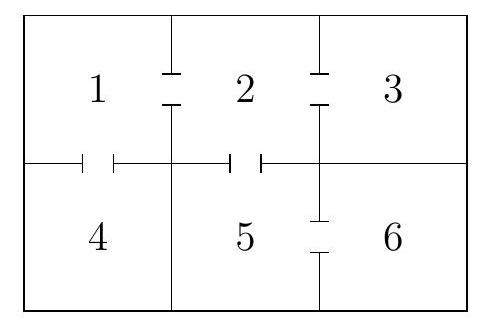
\includegraphics[scale=0.3]{sheet 5 diagram}\end{center}%recreating this in TikZ is left as an exercise to the reader



\question%3
(\emph{Gambler's ruin, symmetric case.}) A gambler starts a game with a bankroll of $\pounds n$ where $n \in\{1,2, \ldots, M-1\}$. At each step of the game, he wins $\pounds 1$ with probability $1 / 2$ and loses $\pounds 1$ with probability $1 / 2$, independently for different steps. The game ends when the gambler's bankroll reaches $\pounds 0$ or $\pounds M$. In lectures we saw that the probability the gambler finishes with $\pounds M$ is $n / M$.
\begin{parts}
\part%3a
What is the expected amount of money that the gambler has at the end of the game?

\part%3b
Suppose we know that the gambler ends the game with $\pounds M$. What is the conditional probability that he won $\pounds 1$ on the first step?

\part%3c
Let $e_{n}$ be the expected length of the game. Find $e_{n}$ for each $n$. For which $n$ is $e_{n}$ largest?
\end{parts}



\question%4
\begin{parts}
\part%4a
Suppose that $X$ has a geometric distribution with parameter $p$. Show that the probability generating function of $X$ is \[
	G_{X}(s)=\frac{p s}{1-(1-p) s}, \qquad \text{for }|s|<\frac{1}{1-p}.
\]

\part%4b
Use this to calculate the mean and variance of $X$.
\end{parts}



\question%5
\begin{parts}
\part%5a
A fair coin is tossed $n$ times. Let $r_{n}$ be the probability that the sequence of tosses never has a head followed by a head. Show that \[
	r_{n}=\frac{1}{2} r_{n-1}+\frac{1}{4} r_{n-2}, \quad n \geq 2.
\] Find $r_{n}$ using the conditions $r_{0}=r_{1}=1$. Check that the value you get for $r_{2}$ is correct.

\part%5b
Let $X$ be the number of coin tosses needed until you first get two heads in a row. (Note that $X \geq 2$.) Find the probability mass function of $X$.

\part%5c
Find the probability generating function of $X$. Use this to calculate the mean of $X$. (You may wish to check that your answer agrees with what you got for Question 6 on Problem Sheet 3!)

\part%5d
Let $Y$ be the number of coin tosses needed until you first see a tail followed by a head. On any two particular coin tosses, the probability of seeing the pattern $\mathrm{TH}$ is $1 / 4$, the same as the probability of seeing the pattern HH. Therefore $\mathbb{P}(Y=2)=$ $\mathbb{P}(X=2)=1 / 4$. Find $\mathbb{P}(Y>n)$ for $n \geq 1$ and compare it to $\mathbb{P}(X>n)$. Is your answer surprising?
\end{parts}



\question%6
(\emph{Optional. If you liked the coupon collector problem on Problem Sheet 3, you might enjoy this question too!}) Consider a symmetric random walk on a cycle with $N$ sites, labelled $0,1,2, \ldots, N-1$. A particle starts at site 0 , and at each step it jumps from its current site $i$ to one of its two neighbours $i+1 \bmod N$ and $i-1 \bmod N$ with equal probability (independently of how it arrived at its current position).
\begin{parts}
\part%6a
Find the expected number of steps until every site has been visited. [\emph{Hint: just after a new site has been visited, what does the set of visited sites look like? The value $e_{1}=M-1$ from Question 3(c) may be useful!}]

\part%6b
For each $k=1, \ldots, N-1$, what is the probability that $k$ is the last site to be visited? [\emph{Hint: before visiting site $k$, the walk must visit either site $k-1$ or site $k+1$. What needs to happen from that point onwards?}]
\end{parts}

\end{questions}

\end{document}
